% !TEX root = ../thesis.tex
\chapter{Konzeption und Definition des Systems}\label{ch:konzeption}
In diesem Kapitel wird das Konzept des Systems vorgestellt sowie definiert, welcher Teil dieses Konzepts umgesetzt wird.
Dafür wird zunächst durch Nutzung eines Komponentendiagramms ein grobes Systemkonzept vorgestellt, welches die einzelnen Komponenten des Systems und deren Zusammenhänge zeigt.
Anhand von Beispielen wird das Konzept des universellen Sensor- und Aktuatorsystems für Smart Gardening erläutert und anschließend werden die einzelnen Komponenten des Systems detailliert beschrieben.

Danach wird definiert, welche Anforderungen des Systems in einem Prototyp umgesetzt werden und welche nicht.
Darauf aufbauend wird definiert, welche Komponenten und Funktionalitäten der Komponenten des Systemkonzepts im Prototyp umgesetzt werden.



\section{Modellierung des Lösungsansatzes}\label{sec:modellierung}
In diesem Abschnitt wird das Systemmodell des universellen Sensor- und Aktuatorsystems für Smart Gardening vorgestellt.
Dafür werden zunächst die übergreifenden Zusammenhänge des Systems mittels eines Diagramms erläutert und mittels eines Beispiels veranschaulicht.
Anschließend werden die einzelnen Komponenten des Systems detailliert beschrieben.

\begin{figure}[!htbp]
	\centering
	%% Creator: Inkscape 1.3.2 (091e20e, 2023-11-25, custom), www.inkscape.org
%% PDF/EPS/PS + LaTeX output extension by Johan Engelen, 2010
%% Accompanies image file 'Grobes-Konzept-Allgemein.eps' (pdf, eps, ps)
%%
%% To include the image in your LaTeX document, write
%%   \input{<filename>.pdf_tex}
%%  instead of
%%   \includegraphics{<filename>.pdf}
%% To scale the image, write
%%   \def\svgwidth{<desired width>}
%%   \input{<filename>.pdf_tex}
%%  instead of
%%   \includegraphics[width=<desired width>]{<filename>.pdf}
%%
%% Images with a different path to the parent latex file can
%% be accessed with the `import' package (which may need to be
%% installed) using
%%   \usepackage{import}
%% in the preamble, and then including the image with
%%   \import{<path to file>}{<filename>.pdf_tex}
%% Alternatively, one can specify
%%   \graphicspath{{<path to file>/}}
%% 
%% For more information, please see info/svg-inkscape on CTAN:
%%   http://tug.ctan.org/tex-archive/info/svg-inkscape
%%
\begingroup%
  \makeatletter%
  \providecommand\color[2][]{%
    \errmessage{(Inkscape) Color is used for the text in Inkscape, but the package 'color.sty' is not loaded}%
    \renewcommand\color[2][]{}%
  }%
  \providecommand\transparent[1]{%
    \errmessage{(Inkscape) Transparency is used (non-zero) for the text in Inkscape, but the package 'transparent.sty' is not loaded}%
    \renewcommand\transparent[1]{}%
  }%
  \providecommand\rotatebox[2]{#2}%
  \newcommand*\fsize{\dimexpr\f@size pt\relax}%
  \newcommand*\lineheight[1]{\fontsize{\fsize}{#1\fsize}\selectfont}%
  \ifx\svgwidth\undefined%
    \setlength{\unitlength}{328.08000183bp}%
    \ifx\svgscale\undefined%
      \relax%
    \else%
      \setlength{\unitlength}{\unitlength * \real{\svgscale}}%
    \fi%
  \else%
    \setlength{\unitlength}{\svgwidth}%
  \fi%
  \global\let\svgwidth\undefined%
  \global\let\svgscale\undefined%
  \makeatother%
  \begin{picture}(1,1.2340893)%
    \lineheight{1}%
    \setlength\tabcolsep{0pt}%
    \put(0,0){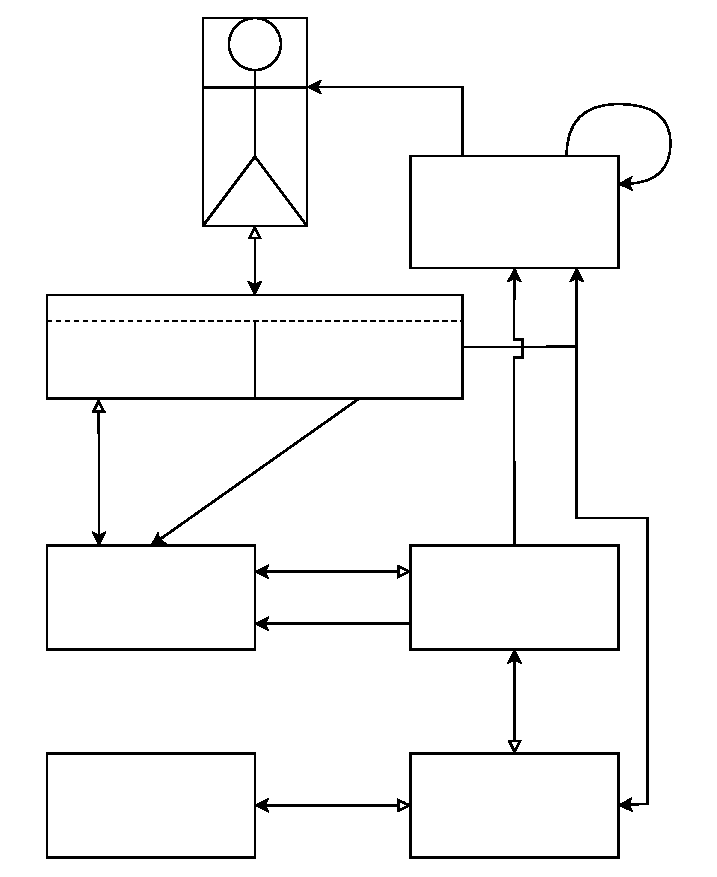
\includegraphics[width=\unitlength]{diagrams/Grobes-Konzept-Allgemein.eps}}%
    \put(0.55798345,0.5730341){\makebox(0,0)[lt]{\lineheight{1.25}\smash{\begin{tabular}[t]{l}Auslöser \&\end{tabular}}}}%
    \put(0.55579089,0.54014579){\makebox(0,0)[lt]{\lineheight{1.25}\smash{\begin{tabular}[t]{l}Herzschlag\end{tabular}}}}%
    \put(0.01638821,0.5730341){\makebox(0,0)[lt]{\lineheight{1.25}\smash{\begin{tabular}[t]{l}Daten-\end{tabular}}}}%
    \put(0.01128367,0.54014579){\makebox(0,0)[lt]{\lineheight{1.25}\smash{\begin{tabular}[t]{l}anfrage\end{tabular}}}}%
    \put(0.13040104,0.5730341){\makebox(0,0)[lt]{\lineheight{1.25}\smash{\begin{tabular}[t]{l}Daten-\end{tabular}}}}%
    \put(0.12676962,0.54014579){\makebox(0,0)[lt]{\lineheight{1.25}\smash{\begin{tabular}[t]{l}antwort\end{tabular}}}}%
    \put(0.376344,0.46340638){\makebox(0,0)[lt]{\lineheight{1.25}\smash{\begin{tabular}[t]{l}Konfiguration\end{tabular}}}}%
    \put(0.40046212,0.43051805){\makebox(0,0)[lt]{\lineheight{1.25}\smash{\begin{tabular}[t]{l}Anfragen\end{tabular}}}}%
    \put(0.74322003,0.24195836){\makebox(0,0)[lt]{\lineheight{1.25}\smash{\begin{tabular}[t]{l}Daten-\end{tabular}}}}%
    \put(0.73958863,0.20907006){\makebox(0,0)[lt]{\lineheight{1.25}\smash{\begin{tabular}[t]{l}antwort\end{tabular}}}}%
    \put(0.7962182,1.11898018){\makebox(0,0)[lt]{\lineheight{1.25}\smash{\begin{tabular}[t]{l}Selbstauslöser\end{tabular}}}}%
    \put(0.83458792,0.75940123){\makebox(0,0)[lt]{\lineheight{1.25}\smash{\begin{tabular}[t]{l}Konfigu-\end{tabular}}}}%
    \put(0.84993578,0.72651293){\makebox(0,0)[lt]{\lineheight{1.25}\smash{\begin{tabular}[t]{l}rieren\end{tabular}}}}%
    \put(0.18192607,0.86683642){\makebox(0,0)[lt]{\lineheight{1.25}\smash{\begin{tabular}[t]{l}Interaktion\end{tabular}}}}%
    \put(0.41981824,0.12136786){\makebox(0,0)[lt]{\lineheight{1.25}\smash{\begin{tabular}[t]{l}Daten-\end{tabular}}}}%
    \put(0.41471372,0.08847956){\makebox(0,0)[lt]{\lineheight{1.25}\smash{\begin{tabular}[t]{l}anfrage\end{tabular}}}}%
    \put(0.42091452,0.05559123){\makebox(0,0)[lt]{\lineheight{1.25}\smash{\begin{tabular}[t]{l}Daten-\end{tabular}}}}%
    \put(0.4172831,0.02270292){\makebox(0,0)[lt]{\lineheight{1.25}\smash{\begin{tabular}[t]{l}antwort\end{tabular}}}}%
    \put(0.4947762,1.14529084){\makebox(0,0)[lt]{\lineheight{1.25}\smash{\begin{tabular}[t]{l}Nachricht\end{tabular}}}}%
    \put(0.14102123,0.08847956){\makebox(0,0)[lt]{\lineheight{1.25}\smash{\begin{tabular}[t]{l}Externe\end{tabular}}}}%
    \put(0.10881808,0.05559123){\makebox(0,0)[lt]{\lineheight{1.25}\smash{\begin{tabular}[t]{l}Datenquellen\end{tabular}}}}%
    \put(0.12382338,0.3757042){\makebox(0,0)[lt]{\lineheight{1.25}\smash{\begin{tabular}[t]{l}Datenbank\end{tabular}}}}%
    \put(0.63653856,0.39105207){\makebox(0,0)[lt]{\lineheight{1.25}\smash{\begin{tabular}[t]{l}Sensor- und\end{tabular}}}}%
    \put(0.62653502,0.35816376){\makebox(0,0)[lt]{\lineheight{1.25}\smash{\begin{tabular}[t]{l}Aktuatorkoffer\end{tabular}}}}%
    \put(0.58751442,0.94138326){\makebox(0,0)[lt]{\lineheight{1.25}\smash{\begin{tabular}[t]{l}Benachrichtigungen\end{tabular}}}}%
    \put(0.376344,0.38885951){\makebox(0,0)[lt]{\lineheight{1.25}\smash{\begin{tabular}[t]{l}Konfiguration\end{tabular}}}}%
    \put(0.41070544,0.35597121){\makebox(0,0)[lt]{\lineheight{1.25}\smash{\begin{tabular}[t]{l}senden\end{tabular}}}}%
    \put(0.65812152,0.10382744){\makebox(0,0)[lt]{\lineheight{1.25}\smash{\begin{tabular}[t]{l}Server für\end{tabular}}}}%
    \put(0.67199629,0.07313167){\makebox(0,0)[lt]{\lineheight{1.25}\smash{\begin{tabular}[t]{l}externe\end{tabular}}}}%
    \put(0.63835429,0.04024334){\makebox(0,0)[lt]{\lineheight{1.25}\smash{\begin{tabular}[t]{l}Datenquellen\end{tabular}}}}%
    \put(0.20663815,0.47409399){\rotatebox{35.00000068}{\makebox(0,0)[lt]{\lineheight{1.25}\smash{\begin{tabular}[t]{l}Konfiguration speichern\end{tabular}}}}}%
    \put(0.62262955,0.24195836){\makebox(0,0)[lt]{\lineheight{1.25}\smash{\begin{tabular}[t]{l}Daten-\end{tabular}}}}%
    \put(0.61752501,0.20907006){\makebox(0,0)[lt]{\lineheight{1.25}\smash{\begin{tabular}[t]{l}anfrage\end{tabular}}}}%
    \put(0.42533389,0.32089033){\makebox(0,0)[lt]{\lineheight{1.25}\smash{\begin{tabular}[t]{l}Daten\end{tabular}}}}%
    \put(0.4172831,0.288002){\makebox(0,0)[lt]{\lineheight{1.25}\smash{\begin{tabular}[t]{l}senden\end{tabular}}}}%
    \put(0.12091139,0.72432038){\makebox(0,0)[lt]{\lineheight{1.25}\smash{\begin{tabular}[t]{l}Dashboard\end{tabular}}}}%
    \put(0.40046212,0.74624592){\makebox(0,0)[lt]{\lineheight{1.25}\smash{\begin{tabular}[t]{l}Konfigurations-\end{tabular}}}}%
    \put(0.43263099,0.71335759){\makebox(0,0)[lt]{\lineheight{1.25}\smash{\begin{tabular}[t]{l}werkzeug\end{tabular}}}}%
    \put(0.229066,0.79667466){\makebox(0,0)[lt]{\lineheight{1.25}\smash{\begin{tabular}[t]{l}Nutzerschnittstelle\end{tabular}}}}%
  \end{picture}%
\endgroup%

	\caption[Darstellung des übergreifenden Systemkonzepts.]{
		Darstellung des übergreifenden Systemkonzepts des universellen Sensor- und Aktuatorsystems für Smart Gardening mit Überblick über die Komponenten und Schnittstellen.
		Dabei sind die Komponenten des Systems in Boxen dargestellt und Pfeile stellen die Datenflüsse zwischen den Komponenten dar.
		Hat ein Pfeil eine nicht ausgefüllte Pfeilspitze, stellt diese die Antwort auf eine Anfrage dar.
		Die zu Anfragen dazugehörige Beschriftung befindet sich über oder links eines Pfeils, die zu Antworten unter oder rechts eines Pfeils.
		Die Komponente Sensor- und Aktuatorkoffer ist selbst in weitere Komponenten unterteilt, die in \cref{pic:koffer-konzept} dargestellt sind.
		}
	\label{pic:systemkonzept}
\end{figure}

Das Systemkonzept besteht aus mehreren Komponenten, die miteinander interagieren, um die verschiedenen Anforderungen und Anwendungsfälle abdecken zu können.
Dieses ist in \cref{pic:systemkonzept} dargestellt und wird anhand der Abbildung im Folgenden erläutert.
Zu diesen Komponenten gehören der Sensor- und Aktuatorkoffer, die Datenbank, die Nutzerschnittstelle, die Benachrichtigungen und der Server für externe Datenquellen.
An oberster Stelle steht dabei der Nutzer, welcher über die Nutzerschnittstelle mit dem System interagiert, wobei diese weiter in ein Dashboard und ein Konfigurationswerkzeug unterteilt ist.
Das Dashboard dient dabei der Anzeige von Informationen und der Steuerung des Systems, während das Konfigurationswerkzeug der Konfiguration des Systems dient.
Hierbei greift das Dashboard auf die Datenbank zu, um die benötigten Informationen anzuzeigen.
Das Konfigurationswerkzeug kann den Sensor- und Aktuatorkoffer, die Benachrichtigungen und den Server für externe Datenquellen konfigurieren.
Der Sensor- und Aktuatorkoffer ist dabei die zentrale Komponente des Systems, welche die Sensorik und Aktuatorik steuert, Regeln ausführt und Daten an die Datenbank sendet.
Gleichzeitig kann der Sensor- und Aktuatorkoffer auch Daten von externen Datenquellen über den Server für externe Datenquellen anfragen, um diese in die Regelverarbeitung einzubeziehen.
Außerdem kann er Benachrichtigungen an den Nutzer auslösen, wenn bestimmte Bedingungen erfüllt sind.
Der Server für externe Datenquellen dient dabei als Schnittstelle zu externen Datenquellen wie Wetterdiensten, um hier eine homogene Schnittstelle für den Sensor- und Aktuatorkoffer zu schaffen.

Anhand eines Beispiels kann das wie folgt aussehen.  % Den Satz einmal verbessern
Ein Nutzer baut das System auf, verbindet verschiedene Sensoren und Aktuatoren mit dem Sensor- und Aktuatorkoffer und konfiguriert das System über das Konfigurationswerkzeug.
Dabei legt er eine Regel zur automatischen Bewässerung an, welche die Bodenfeuchtigkeit und Wetterdaten überwacht und beim Unterschreiten eines Schwellenwerts automatisch die Bewässerung startet und den Nutzer benachrichtigt.
Der Sensor- und Aktuatorkoffer führt diese Regel periodisch aus und sendet in regelmäßigen Abständen einen Herzschlag, um den Betrieb zu bestätigen.
Zur Ausführung dieser Regel greift der Sensor- und Aktuatorkoffer auf den Server für externe Datenquellen zu, um die aktuellen Wetterdaten anzufragen.
Diese werden von dem Server aus einer externen Datenquelle bezogen und an den Sensor- und Aktuatorkoffer weitergeleitet.
Die generierten Messdaten werden an die Datenbank gesendet und durch das Dashboard als digitaler Zwilling seines Gartens für den Nutzer visualisiert.
Wird nun eine Bewässerung durch den Sensor- und Aktuatorkoffer ausgelöst, schickt dieser eine Benachrichtigung an die Benachrichtigungskomponente, welche den Nutzer über die von ihm konfigurierten Quellen informiert.

In den folgenden Abschnitten werden die einzelnen Komponenten näher erläutert und die Schnittstellen zwischen den Komponenten definiert, beginnend mit dem Sensor- und Aktuatorkoffer, der als zentrale Komponente des Systems fungiert.
Darauf folgen die Datenbank, die Nutzerschnittstelle, die Benachrichtigungen und der Server für externe Datenquellen.
Anschließend wird das Systemkonzept zusammengefasst.


\subsection{Erklärung der Systemkomponente Sensor- und Aktuatorkoffer}
In diesem Abschnitt wird die Systemkomponente Sensor- und Aktuatorkoffer genauer erläutert, welche als zentrale Komponente des Systems fungiert.
Dabei wird der Sensor- und Aktuatorkoffer selbst in weitere Komponenten unterteilt, welche die Funktionalität des Sensor- und Aktuatorkoffers bereitstellen.
Diese werden anhand eines Diagramms und eines Beispiels genauer erläutert.

\begin{figure}[!htbp]
	\centering
	%% Creator: Inkscape 1.3.2 (091e20e, 2023-11-25, custom), www.inkscape.org
%% PDF/EPS/PS + LaTeX output extension by Johan Engelen, 2010
%% Accompanies image file 'KofferKonzept.eps' (pdf, eps, ps)
%%
%% To include the image in your LaTeX document, write
%%   \input{<filename>.pdf_tex}
%%  instead of
%%   \includegraphics{<filename>.pdf}
%% To scale the image, write
%%   \def\svgwidth{<desired width>}
%%   \input{<filename>.pdf_tex}
%%  instead of
%%   \includegraphics[width=<desired width>]{<filename>.pdf}
%%
%% Images with a different path to the parent latex file can
%% be accessed with the `import' package (which may need to be
%% installed) using
%%   \usepackage{import}
%% in the preamble, and then including the image with
%%   \import{<path to file>}{<filename>.pdf_tex}
%% Alternatively, one can specify
%%   \graphicspath{{<path to file>/}}
%% 
%% For more information, please see info/svg-inkscape on CTAN:
%%   http://tug.ctan.org/tex-archive/info/svg-inkscape
%%
\begingroup%
  \makeatletter%
  \providecommand\color[2][]{%
    \errmessage{(Inkscape) Color is used for the text in Inkscape, but the package 'color.sty' is not loaded}%
    \renewcommand\color[2][]{}%
  }%
  \providecommand\transparent[1]{%
    \errmessage{(Inkscape) Transparency is used (non-zero) for the text in Inkscape, but the package 'transparent.sty' is not loaded}%
    \renewcommand\transparent[1]{}%
  }%
  \providecommand\rotatebox[2]{#2}%
  \newcommand*\fsize{\dimexpr\f@size pt\relax}%
  \newcommand*\lineheight[1]{\fontsize{\fsize}{#1\fsize}\selectfont}%
  \ifx\svgwidth\undefined%
    \setlength{\unitlength}{369.12000275bp}%
    \ifx\svgscale\undefined%
      \relax%
    \else%
      \setlength{\unitlength}{\unitlength * \real{\svgscale}}%
    \fi%
  \else%
    \setlength{\unitlength}{\svgwidth}%
  \fi%
  \global\let\svgwidth\undefined%
  \global\let\svgscale\undefined%
  \makeatother%
  \begin{picture}(1,1.13784134)%
    \lineheight{1}%
    \setlength\tabcolsep{0pt}%
    \put(0,0){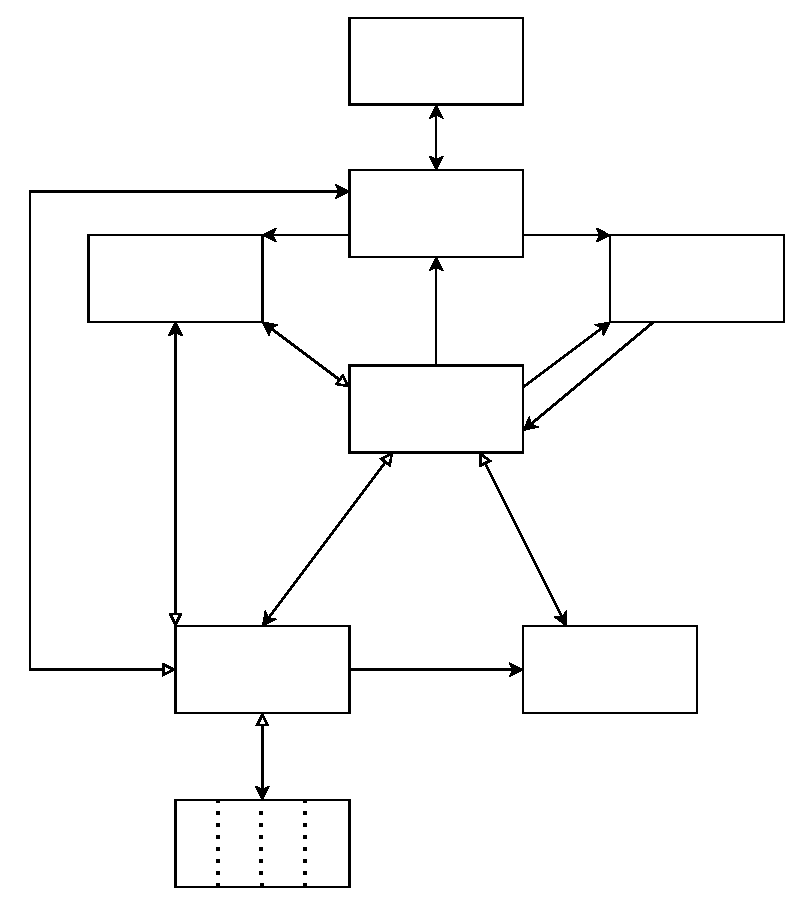
\includegraphics[width=\unitlength]{diagrams/KofferKonzept.eps}}%
    \put(0.36229892,0.75268833){\rotatebox{-37.00000005}{\makebox(0,0)[lt]{\lineheight{1.25}\smash{\begin{tabular}[t]{l}Regel\end{tabular}}}}}%
    \put(0.33445225,0.73951302){\rotatebox{-37.00000005}{\makebox(0,0)[lt]{\lineheight{1.25}\smash{\begin{tabular}[t]{l}anfragen\end{tabular}}}}}%
    \put(0.29118764,0.71969367){\rotatebox{-37.00000005}{\makebox(0,0)[lt]{\lineheight{1.25}\smash{\begin{tabular}[t]{l}Regel senden\end{tabular}}}}}%
    \put(0.66688184,0.62147216){\rotatebox{39.00000116}{\makebox(0,0)[lt]{\lineheight{1.25}\smash{\begin{tabular}[t]{l}Regel auslösen\end{tabular}}}}}%
    \put(0.67293725,0.71663924){\rotatebox{35.99999868}{\makebox(0,0)[lt]{\lineheight{1.25}\smash{\begin{tabular}[t]{l}Job\end{tabular}}}}}%
    \put(0.67209931,0.68230949){\rotatebox{35.99999868}{\makebox(0,0)[lt]{\lineheight{1.25}\smash{\begin{tabular}[t]{l}anlegen\end{tabular}}}}}%
    \put(0.46048854,0.76662729){\makebox(0,0)[lt]{\lineheight{1.25}\smash{\begin{tabular}[t]{l}Daten\end{tabular}}}}%
    \put(0.45394235,0.73934647){\makebox(0,0)[lt]{\lineheight{1.25}\smash{\begin{tabular}[t]{l}senden\end{tabular}}}}%
    \put(0.63499902,0.5214145){\rotatebox{-62.99999795}{\makebox(0,0)[lt]{\lineheight{1.25}\smash{\begin{tabular}[t]{l}Datenantwort\end{tabular}}}}}%
    \put(0.59405085,0.52215864){\rotatebox{-62.99999795}{\makebox(0,0)[lt]{\lineheight{1.25}\smash{\begin{tabular}[t]{l}Datenanfrage\end{tabular}}}}}%
    \put(0.29373901,0.38109393){\rotatebox{52.99999995}{\makebox(0,0)[lt]{\lineheight{1.25}\smash{\begin{tabular}[t]{l}Sensorik anfragen\end{tabular}}}}}%
    \put(0.31158684,0.3594479){\rotatebox{52.99999995}{\makebox(0,0)[lt]{\lineheight{1.25}\smash{\begin{tabular}[t]{l}Aktuatorik auslösen\end{tabular}}}}}%
    \put(0.34596253,0.34802111){\rotatebox{52.99999995}{\makebox(0,0)[lt]{\lineheight{1.25}\smash{\begin{tabular}[t]{l}Ergebnismeldung\end{tabular}}}}}%
    \put(0.44225059,0.29505876){\makebox(0,0)[lt]{\lineheight{1.25}\smash{\begin{tabular}[t]{l}Daten speichern\end{tabular}}}}%
    \put(0.16700054,0.3587181){\rotatebox{90}{\makebox(0,0)[lt]{\lineheight{1.25}\smash{\begin{tabular}[t]{l}Sensor- / Aktuatordefinition\end{tabular}}}}}%
    \put(0.19428137,0.44506678){\rotatebox{90}{\makebox(0,0)[lt]{\lineheight{1.25}\smash{\begin{tabular}[t]{l}anfragen\end{tabular}}}}}%
    \put(0.2390998,0.35871808){\rotatebox{90}{\makebox(0,0)[lt]{\lineheight{1.25}\smash{\begin{tabular}[t]{l}Sensor- / Aktuatordefinition\end{tabular}}}}}%
    \put(0.26638063,0.45106489){\rotatebox{90}{\makebox(0,0)[lt]{\lineheight{1.25}\smash{\begin{tabular}[t]{l}Antwort\end{tabular}}}}}%
    \put(0.34119583,0.97318209){\makebox(0,0)[lt]{\lineheight{1.25}\smash{\begin{tabular}[t]{l}Kommunikation\end{tabular}}}}%
    \put(0.25582146,0.87380195){\makebox(0,0)[lt]{\lineheight{1.25}\smash{\begin{tabular}[t]{l}Konfigurieren\end{tabular}}}}%
    \put(0.66454665,0.86990468){\makebox(0,0)[lt]{\lineheight{1.25}\smash{\begin{tabular}[t]{l}Job anlegen\end{tabular}}}}%
    \put(0.15552789,0.17229505){\makebox(0,0)[lt]{\lineheight{1.25}\smash{\begin{tabular}[t]{l}Ansteuerung\end{tabular}}}}%
    \put(0.32405396,0.17034641){\makebox(0,0)[lt]{\lineheight{1.25}\smash{\begin{tabular}[t]{l}Ergebnis\end{tabular}}}}%
    \put(0.21876703,0.05147997){\makebox(0,0)[lt]{\lineheight{1.25}\smash{\begin{tabular}[t]{l}S1\end{tabular}}}}%
    \put(0.39149484,0.05147997){\makebox(0,0)[lt]{\lineheight{1.25}\smash{\begin{tabular}[t]{l}...\end{tabular}}}}%
    \put(0.03666145,0.29895601){\makebox(0,0)[lt]{\lineheight{1.25}\smash{\begin{tabular}[t]{l}Ansteuerung\end{tabular}}}}%
    \put(0.07268066,0.2658293){\makebox(0,0)[lt]{\lineheight{1.25}\smash{\begin{tabular}[t]{l}Ergebnis\end{tabular}}}}%
    \put(0.32983897,0.05147997){\makebox(0,0)[lt]{\lineheight{1.25}\smash{\begin{tabular}[t]{l}A1\end{tabular}}}}%
    \put(0.70147929,0.28141834){\makebox(0,0)[lt]{\lineheight{1.25}\smash{\begin{tabular}[t]{l}Datenbank\end{tabular}}}}%
    \put(0.26185003,0.30869916){\makebox(0,0)[lt]{\lineheight{1.25}\smash{\begin{tabular}[t]{l}Sensor \&\end{tabular}}}}%
    \put(0.26602133,0.28141834){\makebox(0,0)[lt]{\lineheight{1.25}\smash{\begin{tabular}[t]{l}Aktuator\end{tabular}}}}%
    \put(0.24814873,0.2521889){\makebox(0,0)[lt]{\lineheight{1.25}\smash{\begin{tabular}[t]{l}Schnittstelle\end{tabular}}}}%
    \put(0.49032692,1.08620265){\makebox(0,0)[lt]{\lineheight{1.25}\smash{\begin{tabular}[t]{l}Restliches\end{tabular}}}}%
    \put(0.50402824,1.05697319){\makebox(0,0)[lt]{\lineheight{1.25}\smash{\begin{tabular}[t]{l}System\end{tabular}}}}%
    \put(0.81644849,0.78806221){\makebox(0,0)[lt]{\lineheight{1.25}\smash{\begin{tabular}[t]{l}Scheduler\end{tabular}}}}%
    \put(0.12337549,0.79001084){\makebox(0,0)[lt]{\lineheight{1.25}\smash{\begin{tabular}[t]{l}Definitionen\end{tabular}}}}%
    \put(0.45397279,0.62048002){\makebox(0,0)[lt]{\lineheight{1.25}\smash{\begin{tabular}[t]{l}Regelausführer\end{tabular}}}}%
    \put(0.27235437,0.05147997){\makebox(0,0)[lt]{\lineheight{1.25}\smash{\begin{tabular}[t]{l}S2\end{tabular}}}}%
    \put(0.46310699,0.87575058){\makebox(0,0)[lt]{\lineheight{1.25}\smash{\begin{tabular}[t]{l}Schnittstelle\end{tabular}}}}%
  \end{picture}%
\endgroup%

	\caption[Darstellung der Systemkomponente Sensor- und Aktuatorkoffer.]{
		Darstellung der Systemkomponente Sensor- und Aktuatorkoffer mit Überblick über die Komponenten und Schnittstellen.
		Dabei sind die Komponenten des Systems in Boxen dargestellt und Pfeile stellen die Datenflüsse zwischen den Komponenten dar.
		Hat ein Pfeil eine nicht ausgefüllte Pfeilspitze, stellt diese die Antwort auf eine Anfrage dar.
		Die zu Anfragen dazugehörige Beschriftung befindet sich über oder links eines Pfeils, die zu Antworten unter oder rechts eines Pfeils.
		}
	\label{pic:koffer-konzept}
\end{figure}

Der Sensor- und Aktuatorkoffer besteht aus unterschiedlichen Komponenten und Schnittstellen, welche die Funktionalität des Sensor- und Aktuatorkoffers bereitstellen.
Diese sind in \cref{pic:koffer-konzept} dargestellt und werden im Folgenden anhand der Abbildung erläutert.
Die zentrale Komponente des Sensor- und Aktuatorkoffers ist der Regelausführer, welcher durch die Ausführung von Regeln die Steuerung des Sensor- und Aktuatorkoffers übernimmt.
Die Ausführung einer Regel wird dabei durch den Scheduler gesteuert, welcher die zeitliche Planung der Regelausführung übernimmt.
Außerdem greift der Regelausführer auf die Sensor- und Aktuatorschnittstelle zu, um die Sensorik und Aktuatorik anzusteuern und Messdaten zu erfassen.
In den Definitionen werden die unterschiedlichen Regeln und die unterschiedlichen Sensoren und Aktuatoren definiert, welche im Sensor- und Aktuatorkoffer verwendet werden.
Die Komponenten fragen diese Definitionen an, wenn sie benötigt werden, um ihre Funktion auszuüben.
Stehen die Messdaten zur Verfügung, werden diese in der Datenbank gespeichert, um sie für die weitere Verarbeitung bereitzustellen.

Zur Veranschaulichung mittels eines Beispiels wird das vorherige Beispiel mit der Bewässerungsregel für die Sensor- und Aktuatorkofferkomponente fortgeführt.
Der Sensor- und Aktuatorkoffer erfragt die Konfiguration über die Schnittstelle und legt die Regel und die Sensor- und Aktuatordefinitionen in den Definitionen ab.
Gleichzeitig wird im Scheduler die Regel als Job angelegt, der periodisch ausgeführt wird.
Löst der Scheduler diese Regel nun aus, greift der Regelausführer auf die Definitionen zu und lädt die Regeldefinition.
In diesem Fall beinhaltet die Regeldefinition die Bedingung, dass die Bodenfeuchtigkeit unter einen Schwellenwert fällt und die Wetterdaten keinen Regen vorhersagen, um eine Bewässerung auszulösen und eine Benachrichtigung zu verschicken.
Der Regelausführer fragt nun die Sensor- und Aktuatorschnittstelle ab, um die aktuellen Messdaten zu erhalten.
Diese holt sich die Definition für den Bodenfeuchtigkeitssensor und den Wetterdienst von den Definitionen und fragt die Sensoren ab.
Das Ergebnis wird in der Datenbank gespeichert und der Regelausführer kann die Bedingung nun prüfen.
Für dieses Beispiel wird angenommen, dass die Bedingung erfüllt ist und die Bewässerung ausgelöst wird.
Der Regelausführer weist nun die Sensor- und Aktuatorschnittstelle an, die Bewässerung zu starten, wo der Vorgang analog zum Vorgang für die Sensorik läuft.
Sobald dies beendet ist, löst der Regelausführer über die Schnittstelle zum restlichen System eine Benachrichtigung aus.

Im Folgenden werden die einzelnen Komponenten des Sensor- und Aktuatorkoffers detailliert erläutert, beginnend mit dem Scheduler.
Darauf folgen der Regelausführer, die Schnittstelle, die Definitionen, die Datenbank und die Sensor- und Aktuatorschnittstelle.

\subsubsection{Erklärung der Kofferkomponente Scheduler}
Der Scheduler ist die Komponente des Sensor- und Aktuatorkoffers, die den Takt angibt und steuert, wann welche Regeln ausgeführt werden.
Eine solche einmalige oder periodische Anlegung von Regeln wird als Job bezeichnet.
Dafür bietet der Scheduler eine Schnittstelle an, über die Regeln angelegt, geändert und gelöscht werden können.
Die Komponente kennt dabei nur die ID der Regel und den Zeitpunkt, zu dem die Regel ausgeführt werden soll, wobei dieser auch periodisch sein kann.
Dabei ist es wichtig, dass der Scheduler die Zeitzone des Systems berücksichtigt, um die Regeln korrekt auszuführen.
Soll eine Regel ausgeführt werden, ruft der Scheduler den Regelausführer mit der ID der Regel auf, um die Regel auszuführen.
Außerdem muss der Scheduler so funktionieren, dass er auch bei einem Schlafmodus des Systems zum Sparen von Energie weiterhin Regeln ausführen kann.

\subsubsection{Erklärung der Kofferkomponente Regelausführer}
Der Regelausführer stellt die zentrale Komponente des Sensor- und Aktuatorkoffers dar, welche durch die Ausführung von Regeln die Steuerung des Sensor- und Aktuatorkoffers übernimmt.
Die Regeln müssen ein bestimmtes Format einhalten, welches in \cref{sec:definitionsformat} definiert ist.
Der Regelausführer ist zwar mit allen weiteren Komponenten verbunden, weist jedoch nur eine Schnittstelle auf.
Über diese kann durch Übergabe der ID der Regel die Regelausführung gestartet werden.
Diese beginnt mit dem Laden der Regeldefinition aus den Definitionen durch Übergabe der ID der Regel.
Anschließend wird die Regel ausgeführt, welche mehrere Schritte umfassen kann.
Zunächst kann eine Messung mit einem Sensor durchgeführt werden, wofür die Sensor- und Aktuatorschnittstelle mit der ID des Sensors aufgerufen wird.
Der Regelausführer wartet darauf, dass die Messung abgeschlossen ist und fährt dann mit der weiteren Verarbeitung der Regel fort.
Eine Regel kann auch eine Aktion mit einem Aktuator auslösen, wofür die Sensor- und Aktuatorschnittstelle mit der ID des Aktuators aufgerufen wird.
Auch hier wartet der Regelausführer darauf, dass die Aktion abgeschlossen ist und fährt dann mit der weiteren Verarbeitung der Regel fort.
Sollte die Regel eine Benachrichtigung auslösen, wird die Benachrichtigungskomponente des Gesamtsystems über die Schnittstelle mit der ID der Benachrichtigung aufgerufen.
Weiterhin kann die Regel selbst einen Job im Scheduler anlegen.
Die letzte Option ist das Abrufen von Daten aus der lokalen Datenbank, die zum einen für die Verarbeitung der Regel verwendet und zum anderen an die Datenbank des Gesamtsystems gesendet werden können.

\subsubsection{Erklärung der Kofferkomponente Sensor- und Aktuatorkofferschnittstelle}
Die Schnittstelle des Sensor- und Aktuatorkoffers stellt die Verbindung zu den anderen Komponenten des Gesamtsystems her.
Dabei bietet sie dem Sensor- und Aktuatorkoffer unterschiedliche Methoden an, um die verschiedenen Funktionen zu realisieren.
Welche Kommunikationsarten genau unterstützt werden, ist ein Implementierungsdetail.
Gleichzeitig ist die Schnittstelle auch für den Herzschlag des Sensor- und Aktuatorkoffers zuständig, welcher periodisch an das Gesamtsystem gesendet wird, um den Betrieb zu bestätigen.
Um eine Nachricht zu senden, muss der Schnittstelle die Komponente und die Nachricht übergeben werden.
Die Antwort wird der Komponente zurückgegeben, welche die Nachricht gesendet hat.

\subsubsection{Erklärung der Kofferkomponente Definitionen}
Die Definitionen des Sensor- und Aktuatorkoffers enthalten die Definitionen für die Regeln, Sensoren und Aktuatoren, welche im Sensor- und Aktuatorkoffer verwendet werden.
Sie werden in einem Schlüssel-Werte-Format abgelegt, wobei der Schlüssel die ID der Definition ist und der Wert die Definition selbst.
Das genaue Format für die Regeln und die Sensor- und Aktuatordefinitionen ist in \cref{sec:definitionsformat} definiert.
Die Definitionen werden über die Schnittstelle angefragt, wobei die ID der Definition übergeben wird.
Außerdem können die Definitionen auch über die Schnittstelle konfiguriert, also angelegt, geändert und gelöscht werden.

\subsubsection{Erklärung der Kofferkomponente Datenbank}
Die Datenbank des Sensor- und Aktuatorkoffers dient dazu, die Messdaten der Sensoren und Ergebnisse der Aktuatoren temporär zu speichern.
Diese Daten werden zum einen für die Verarbeitung der Regeln benötigt und zum anderen an die Datenbank des Gesamtsystems gesendet, um sie dort dauerhaft zu speichern.
Die lokale Datenbank kann die Daten aufgrund der knappen lokalen Ressourcen nur temporär speichern, wobei die Speicherdauer von der Implementierung und den genutzten Regeln abhängt.
Wird der Speicherplatz knapp, werden die ältesten Daten gelöscht, um Platz für neue Daten zu schaffen.
Zwei Schnittstellen werden für die Datenbank benötigt, eine zum Speichern der Daten und eine zum Abrufen der Daten.
Für das Abfragen der Daten kann zum einen die Datenquelle und zum anderen der Zeitraum angegeben werden, für den die Daten abgefragt werden sollen.

\subsubsection{Erklärung der Kofferkomponente Sensor- und Aktuatorschnittstelle}
Die Sensor- und Aktuatorschnittstelle des Sensor- und Aktuatorkoffers dient dazu, die Sensorik und Aktuatorik anzusteuern und Messdaten zu erfassen.
Dafür kann der Nutzer bei der Konfiguration des Systems unterschiedliche Sensoren und Aktuatoren an den Sensor- und Aktuatorkoffer anschließen und diese über das Konfigurationswerkzeug konfigurieren.
Auch externe Datenquellen können virtuell als Sensoren und Aktuatoren an den Sensor- und Aktuatorkoffer angeschlossen werden, sodass deren Nutzung identisch zu lokalen Sensoren und Aktuatoren ist.
Die Sensor- und Aktuatorschnittstelle bietet dafür eine Schnittstelle an, über die durch Übergabe der ID des Sensors oder Aktuators die Messung oder Aktion gestartet werden kann.
Anschließend fragt sie die Definition des Sensors oder Aktuators aus den Definitionen ab und führt die Messung oder Aktion durch Ansteuerung des Sensors oder Aktuators aus, woraufhin die Messdaten zurückgegeben werden.


\subsection{Erklärung der Systemkomponente Datenbank}
Die Datenbank des Gesamtsystems dient dazu, die Messdaten der Sensoren, Ergebnisse der Aktuatoren und die aktuelle Konfiguration dauerhaft zu speichern.
Diese Daten können durch den Nutzer zur Analyse genutzt werden und ermöglichen durch die dauerhafte Speicherung auch eine spätere Analyse und die Analyse von längeren Zeiträumen.
Dabei weist diese Komponente zwei Schnittstellen auf, eine zum Speichern der Daten und eine zum Abrufen der Daten.
Für das Speichern der Daten können größere Datenpakete übergeben werden, die viele unterschiedliche Daten enthalten können.
Für das Abrufen der Daten kann zum einen die Datenquelle und zum anderen der Zeitraum angegeben werden, für den die Daten abgefragt werden sollen.


\subsection{Erklärung der Systemkomponente Nutzerschnittstelle}
Die Nutzerschnittstelle des Systems dient dazu, dem Nutzer die Interaktion mit dem System zu ermöglichen.
Zu dieser gehört zum einen die Möglichkeit, die Daten des Systems zu visualisieren und zum anderen die Möglichkeit, das System zu konfigurieren.
Für die Visualisierung der Daten wird ein Dashboard bereitgestellt, welches dem Nutzer eine Art digitalen Zwilling seines Gartens anzeigt.
Dafür greift das Dashboard auf die Datenbank zu, um die benötigten Informationen anzuzeigen.
Für die Konfiguration des Systems wird ein Konfigurationswerkzeug bereitgestellt, welches dem Nutzer ermöglicht, den Sensor- und Aktuatorkoffer, also die Sensoren, Aktuatoren und Regeln, die Benachrichtigungen und den Server für externe Datenquellen zu konfigurieren.


\subsection{Erklärung der Systemkomponente Benachrichtigungen}
Die Benachrichtigungskomponente des Systems dient dazu, den Nutzer über bestimmte Ereignisse zu informieren.
Über eine Schnittstelle zur Konfiguration kann der Nutzer festlegen, über welche Kanäle er benachrichtigt werden möchte.
Beispiele hierfür sind E-Mail, SMS, Push-Benachrichtigungen oder RSS-Feeds.
Ausgelöst werden können Benachrichtigungen durch den Sensor- und Aktuatorkoffer selbst oder den Ausfall des Herzschlags des Sensor- und Aktuatorkoffers.
Für das Auslösen einer Benachrichtigung bietet die Komponente eine Schnittstelle an, über die durch Übergabe einer Priorität und einer Nachricht die Benachrichtigung ausgelöst werden kann.
Außerdem bietet die Komponente eine Schnittstelle für den Herzschlag des Sensor- und Aktuatorkoffers an, wobei über die Konfiguration festgelegt werden kann, wie lange der Herzschlag ausfallen darf, bevor eine Benachrichtigung durch die Komponente selbst ausgelöst wird.
Dadurch kann sichergestellt werden, dass der Nutzer über einen Ausfall des Sensor- und Aktuatorkoffers informiert wird und entsprechend reagieren kann.


\subsection{Erklärung der Systemkomponente Server für externe Datenquellen}
Der Server für externe Datenquellen dient dazu, eine homogene Schnittstelle für den Sensor- und Aktuatorkoffer zu externen Datenquellen bereitzustellen.
Zu möglichen externen Datenquellen gehören etwa Wetterdienste, um aktuelle Wetterdaten abzufragen, und IoT-Sensoren, die nicht direkt mit dem Sensor- und Aktuatorkoffer selbst verbunden werden können.
Diese externen Datenquellen können durch den Nutzer über das Konfigurationswerkzeug konfiguriert werden.
Der Server bietet eine Schnittstelle an, über die der Sensor- und Aktuatorkoffer die Daten anfragen kann, indem er die ID der Datenquelle übergibt.
Die Daten werden dann von der externen Datenquelle bezogen und an den Sensor- und Aktuatorkoffer weitergeleitet.


\subsection{Erklärung des Definitionsformats}\label{sec:definitionsformat}
Die Definitionen des Systems, also die Regeln, Sensoren und Aktuatoren, sind in einem bestimmten Format abzulegen, um eine einheitliche Verarbeitung zu gewährleisten.
Dabei wird ein Schlüssel-Werte-Format verwendet.

Für die Sensor- und Aktuatordefinitionen wird zunächst die ID angegeben und danach, ob es sich um einen Sensor oder Aktuator handelt.
Darauf folgen ein Anzeigename, die technischen Daten, wie die Art des Sensors oder Aktuators, die Anschlüsse, die benötigte Spannung und das Protokoll.
Zum Schluss kommen noch die zur Verfügung stehenden Befehle, die der Sensor oder Aktuator ausführen kann.
Die genauen relevanten Schlüssel und Werte sind von der Art des Sensors oder Aktuators abhängig.

Auch für die Regeldefinition wird zunächst die ID angegeben, gefolgt von einem Anzeigenamen und einer Beschreibung.
Eine Regel besteht dabei aus einer Liste von Aktionen, also Sensor- und Aktuatorausführungen und schachtelbaren Wenn-Dann-Sonst-Bedingungen.
Dabei können die Wenn-Bedingungen Konstanten und Messwerte aus der lokalen Datenbank enthalten, wodurch die vorherigen Messungen genutzt werden können.
Der Dann-Sonst Teil besteht aus einer Liste von Aktionen, die ausgeführt werden, wenn die Wenn-Bedingungen erfüllt oder nicht erfüllt sind oder weiteren Wenn-Dann-Sonst-Bedingungen.
Auch das Senden von Benachrichtigungen oder das Anlegen von Jobs im Scheduler sind mögliche Aktionen.


\subsection{Zusammenfassung des Systemkonzepts}
In diesem Abschnitt wurde das Systemkonzept des universellen Sensor- und Aktuatorsystems für Smart Gardening vorgestellt.
Das übergreifende Konzept wird mittels eines Diagramms und eines Beispiels erläutert, wobei die Hauptkomponenten des Systems detailliert beschrieben werden.
Diese umfassen den Sensor- und Aktuatorkoffer, die Datenbank, die Nutzerschnittstelle, die Benachrichtigungen und den Server für externe Datenquellen.
Der Nutzer interagiert über die Nutzerschnittstelle in Form eines Dashboards und Konfigurationswerkzeugs mit dem System, wobei der Sensor- und Aktuatorkoffer zentrale Daten verarbeitet und steuert.
Externe Datenquellen können integriert und Benachrichtigungen bei bestimmten Bedingungen ausgelöst werden.
Die einzelnen Komponenten interagieren über definierte Schnittstellen miteinander, um eine reibungslose und effiziente Systemintegration zu gewährleisten.
Außerdem können Regeln definiert werden, über die der Sensor- und Aktuatorkoffer automatisiert Aktionen ausführen kann.
Im nächsten Abschnitt wird basierend auf dem Systemkonzept die Definition des zu realisierenden Systems vorgenommen, wobei die Kernfunktionalität und die Abgrenzung des Systems definiert werden.



\section{Definition des zu realisierenden Systems}\label{sec:realisieren}
In diesem Abschnitt wird definiert, welche Anforderungen und Funktionalitäten des Systems im Prototyp umgesetzt und nicht umgesetzt werden.
Dafür werden zunächst die Anforderungen genannt, die umgesetzt werden.
Dann wird für jede Komponente des Systems definiert, welche Funktionalitäten umgesetzt werden.
Grundsätzlich wird jede Komponente mindestens rudimentär umgesetzt, wobei der Grad der Umsetzung sich nach der Wichtigkeit der Komponente richtet, orientiert an den in der Analyse definierten Anforderungen.

Zunächst weist das System unterschiedliche Anforderungen auf, die in der Analyse definiert wurden.
Für den Prototyp werden die Anforderungen Messung mittels Sensoren, Konfiguration des Systems, Regeldefinition und Dashboard umgesetzt.
Dementsprechend werden die funktionalen Anforderungen Steuerung von Aktuatoren, autonomer Betrieb und Benachrichtigung des Nutzers nicht oder nicht vollständig umgesetzt.
Von den nicht funktionalen Anforderungen wird nur der Preis umgesetzt.
Aus der Umsetzung dieser Anforderungen ergibt sich für die Funktionalitäten der einzelnen Komponenten des Systems, dass jeweils die folgenden Funktionalitäten umgesetzt oder nicht umgesetzt werden.

Der Sensor- und Aktuatorkoffer stellt die zentrale Komponente des Systems dar und ist in Subkomponenten unterteilt, die in \cref{pic:koffer-konzept} dargestellt sind.
Er dient der Steuerung unterschiedlicher Sensorik und Aktuatorik durch die Ausführung von Regeln.
Für den Prototyp wird die Steuerung der Sensorik umgesetzt, die Steuerung der Aktuatorik jedoch nicht.
Heruntergebrochen auf die Subkomponenten bedeutet das, dass für diese jeweils die folgenden Funktionalitäten umgesetzt werden:

Die Subkomponente Scheduler gibt den Takt für die Ausführung der Regeln an, weshalb diese Funktionalität des Schedulers umgesetzt wird.
Das bedeutet also, dass Jobs angelegt werden können und die Regeln zu den entsprechenden Zeitpunkten ausgeführt werden.
Nicht umgesetzt wird hingegen die Funktionalität, dass der Scheduler auch bei einem Schlafmodus des Systems weiterhin Regeln ausführen kann.

Der Regelausführer stellt die Kernkomponente des Koffers dar, die die Regeln ausführt und die Steuerung übernimmt.
Hierfür wird die grundlegende Wenn-Dann-Sonst-Struktur umgesetzt, wobei die Bedingungen aus Konstanten und Messwerten bestehen können und die Aktionen Sensormessungen und Benachrichtigungen umfassen.
Nicht umgesetzt wird hingegen, dass die Aktuatorik als Aktion eingesetzt werden kann.

Die Schnittstelle stellt die Verbindung zu den anderen Komponenten des Systems her.
Für den Prototyp wird die Schnittstelle so umgesetzt, dass sie die Kommunikation mit allen anderen Komponenten ermöglicht.
Nicht umgesetzt wird hingegen der Herzschlag des Sensor- und Aktuatorkoffers, der hauptsächlich für die Benachrichtigung relevant ist.

Die Definitionen enthalten die Definitionen für die Regeln, Sensoren und Aktuatoren, die im Sensor- und Aktuatorkoffer verwendet werden.
Für den Prototyp wird die Definition der Sensoren und Regeln umgesetzt, wobei die Definitionen über die Schnittstelle konfiguriert werden können.
Nicht umgesetzt wird hingegen die Definition der Aktuatoren.

Die Datenbank dient dazu, die Messdaten der Sensoren und Ergebnisse der Aktuatoren temporär zu speichern.
Für den Prototyp wird die Speicherung der Daten und das Abrufen der Daten umgesetzt, wobei die Datenquelle und der Zeitraum angegeben werden können.
Nicht umgesetzt wird hingegen das automatische Freigeben von Speicherplatz, wenn dieser knapp wird, und das Speichern von Aktuatorikergebnissen.

Die Sensor- und Aktuatorschnittstelle dient dazu, die Sensorik und Aktuatorik anzusteuern und Messdaten zu erfassen.
Für den Prototyp wird die Ansteuerung der Sensoren über ein Protokoll umgesetzt, wobei die Messdaten in der Datenbank gespeichert werden.
Als virtueller Sensor wird weiterhin ein Wetterdienst integriert, um die Wetterdaten abzufragen.
Nicht umgesetzt wird hingegen die Ansteuerung der Aktuatoren und die Ansteuerung anderer externer Datenquellen als dem Wetterdienst.

Die nächste Systemkomponente ist die Datenbank, die die Messdaten der Sensoren, Ergebnisse der Aktuatoren und die aktuelle Konfiguration dauerhaft speichert.
Für den Prototyp wird eine vorübergehende Speicherung der Daten und das Abrufen der Daten umgesetzt, wobei die Datenquelle und der Zeitraum angegeben werden können.
Nicht umgesetzt wird hingegen die Speicherung von Aktuatorikergebnissen.

Die Nutzerschnittstelle dient dazu, dem Nutzer die Interaktion mit dem System zu ermöglichen durch Visualisierung der Daten und Konfiguration des Systems.
Für den Prototyp wird ein simples Dashboard umgesetzt, welches die aktuellen Messdaten anzeigt und ein Konfigurationswerkzeug, welches das Laden einer Konfiguration ermöglicht, die Regeldefinitionen und Sensorikdefinitionen beinhaltet.
Für das Dashboard werden komplexere Visualisierungen nicht unterstützt und für das Konfigurationswerkzeug wird die Konfiguration von Aktuatoren, Benachrichtigungen und dem Server für externe Datenquellen nicht unterstützt.

Die Systemkomponente Benachrichtigungen dient dazu, den Nutzer über bestimmte Ereignisse zu informieren.
Für den Prototyp wird das generelle Auslösen von Benachrichtigungen umgesetzt, wobei ein Benachrichtigungskanal umgesetzt wird.
Weitere Benachrichtigungskanäle wie E-Mail, SMS oder Push-Benachrichtigungen werden nicht unterstützt.
Außerdem wird die Selbstauslösung bei Ausfall des Herzschlags des Sensor- und Aktuatorkoffers nicht umgesetzt.

Der Server für externe Datenquellen dient dazu, eine homogene Schnittstelle für den Sensor- und Aktuatorkoffer zu externen Datenquellen bereitzustellen.
Für den Prototyp wird für den Server eine Datenquelle umgesetzt, die es ermöglicht, Wetterdaten abzufragen.
Weitere Datenquellen wie IoT-Sensoren werden nicht unterstützt.

Zusammengefasst werden vier von sieben funktionalen Anforderungen vollständig umgesetzt, sowie eine nicht funktionale Anforderung.
Außerdem werden alle Komponenten des Systems mindestens rudimentär umgesetzt, je nach Wichtigkeit der Komponente.



\section{Zusammenfassung der Konzeption und Definition des Systems}
In diesem Kapitel wurde das Systemkonzept des universellen Sensor- und Aktuatorsystems für Smart Gardening vorgestellt und definiert, welche Anforderungen und Funktionalitäten des Systems im Prototyp umgesetzt werden.
Das Systemkonzept besteht aus mehreren Komponenten, die miteinander interagieren, um die verschiedenen Anforderungen und Anwendungsfälle abdecken zu können.
Zu den Komponenten gehören der Sensor- und Aktuatorkoffer, die Datenbank, die Nutzerschnittstelle, die Benachrichtigungen und der Server für externe Datenquellen, wobei der Sensor- und Aktuatorkoffer als zentrale Komponente des Systems fungiert und in Subkomponenten unterteilt ist.
Für den Prototyp werden vier von sieben funktionalen Anforderungen vollständig umgesetzt, sowie eine nicht funktionale Anforderung.
Dafür werden alle Komponenten des Systems mindestens rudimentär umgesetzt, je nach Wichtigkeit der Komponente.

Im nächsten Kapitel wird die Umsetzung des Systems beschrieben, wobei die Implementierung der einzelnen Komponenten des Systems und die Integration der Komponenten beschrieben werden.